\section{Kaka Kamaludin (1174067)}
\subsection{Instalasi Map Server}
\begin{enumerate}

    \item click I Agree
    \hfill\break
    \begin{figure}[H]
		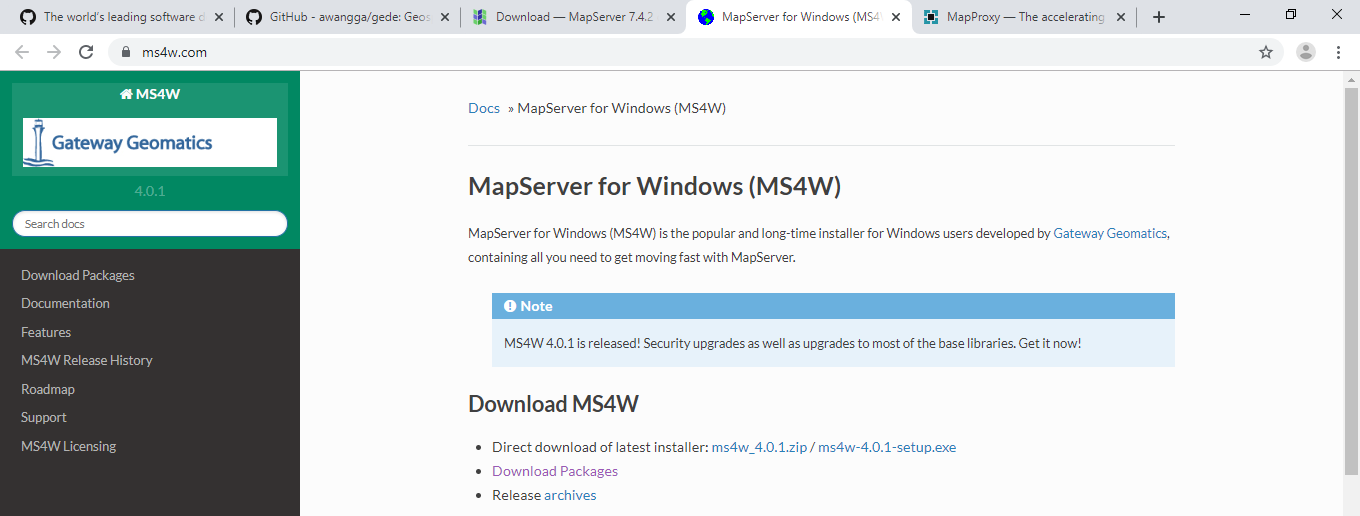
\includegraphics[width=4cm]{figures/tugas4/1174067/1.png}
		\centering
		\caption{Install MS4W 4.0.1}
    \end{figure}
    \hfill\break

    \item type install full, next
    \hfill\break
    \begin{figure}[H]
		
\includegraphics[width=4cm]{figures/tugas4/1174067/2.png}
		\centering
		\caption{Install MS4W 4.0.1}
    \end{figure}
    \hfill\break

    \item Destination Root
    \hfill\break
    \begin{figure}[H]
		
\includegraphics[width=4cm]{figures/tugas4/1174067/3.png}
		\centering
		\caption{Install MS4W 4.0.1}
    \end{figure}
    \hfill\break

    \item Apache port 8080
    \hfill\break
    \begin{figure}[H]
		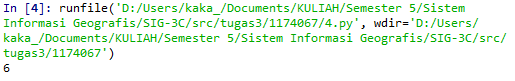
\includegraphics[width=4cm]{figures/tugas4/1174067/4.png}
		\centering
		\caption{Install MS4W 4.0.1}
    \end{figure}
    \hfill\break

    \item tunggu sampai download selesai
    \hfill\break
    \begin{figure}[H]
		
\includegraphics[width=4cm]{figures/tugas4/1174067/5.png}
		\centering
		\caption{Install MS4W 4.0.1}
    \end{figure}
    \hfill\break

    \item tunggu hingga proses Extract selesai
    \hfill\break
    \begin{figure}[H]
		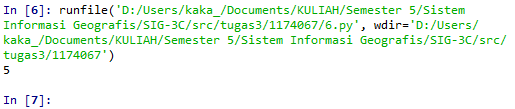
\includegraphics[width=4cm]{figures/tugas4/1174067/6.png}
		\centering
		\caption{Install MS4W 4.0.1}
    \end{figure}
    \hfill\break

\end{enumerate}

\subsection{Instalasi MapProxy}
\begin{enumerate}
  \item Buka CMD
  \item ketik pip install MapProxy
  \hfill\break
  \begin{figure}[H]
  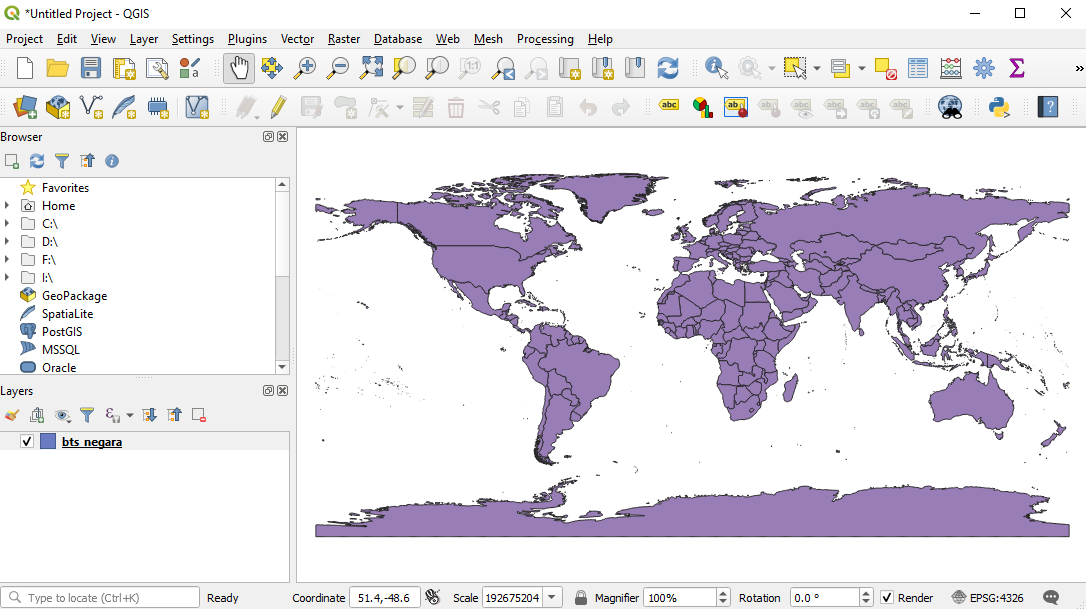
\includegraphics[width=4cm]{figures/tugas4/1174067/9.png}
  \centering
  \caption{Instalasi MapProxy}
  \end{figure}
\end{enumerate}

\subsection{Membuka map menggunakan MapProxy}
\begin{enumerate}
  \item git clone https://github.com/awangga/gede.git
  \item cd gede
  \item mkdir tmp
  \hfill\break
  \begin{figure}[H]
  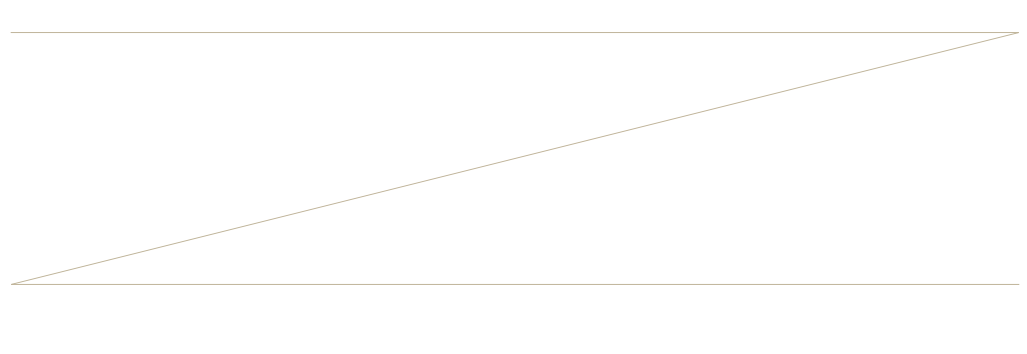
\includegraphics[width=4cm]{figures/tugas4/1174067/7.png}
  \centering
  \caption{Buat folder tmp}
  \end{figure}

  \item edit file agm.yaml di dalam folder mapproxy
  \hfill\break
  \begin{figure}[H]
  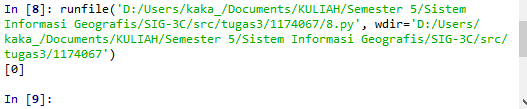
\includegraphics[width=4cm]{figures/tugas4/1174067/8.png}
  \centering
  \caption{File agm.yaml}
  \end{figure}

  \item masih pada folder mappsroxy, jalankan perintah "mapproxy-util serve-develop ./agm.yaml" untuk memulai mapproxy
  \hfill\break
  \begin{figure}[H]
  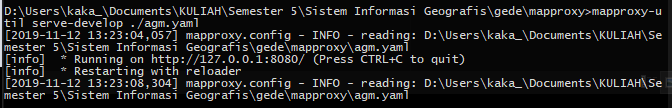
\includegraphics[width=4cm]{figures/tugas4/1174067/9,5.png}
  \centering
  \caption{Buka Folder gede}
  \end{figure}

  \item Buka browser lalu ketikkan http://127.0.0.1:8080/
  \hfill\break
  \begin{figure}[H]
  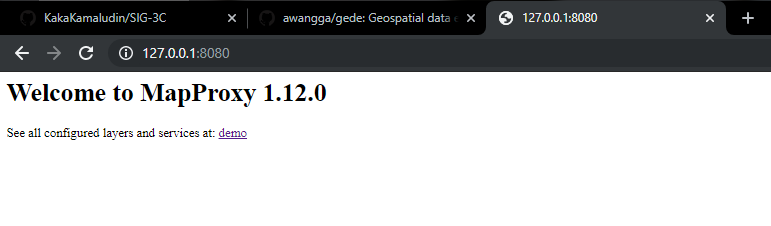
\includegraphics[width=4cm]{figures/tugas4/1174067/9,6.png}
  \centering
  \caption{Buka mapproxy pada browser}
  \end{figure}

  \item lalu klik demo untuk melihat map
  \item lalu klik png pada agm, maka mapproxy akan menampilkan map
  \hfill\break
  \begin{figure}[H]
  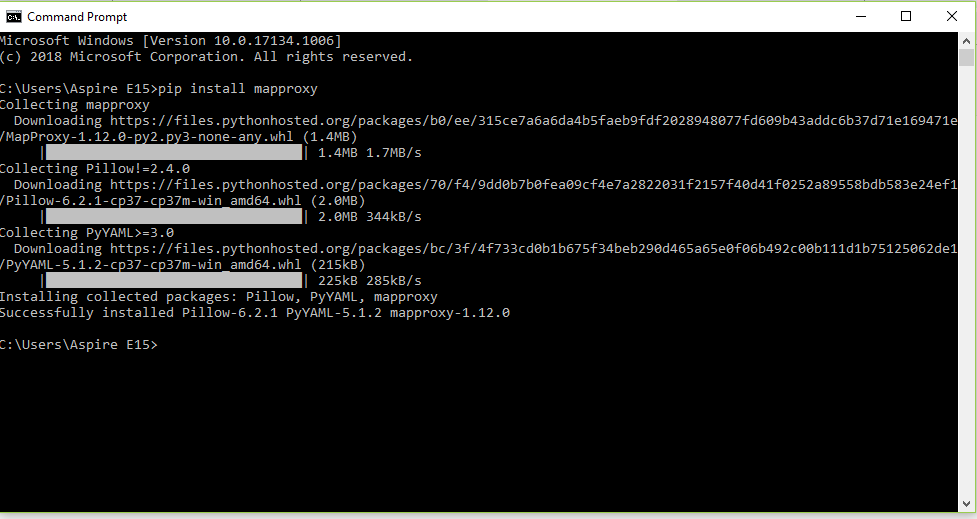
\includegraphics[width=4cm]{figures/tugas4/1174067/10.png}
  \centering
  \caption{MapProxy menampilkan map}
  \end{figure}

\end{enumerate}

\subsection{Link Youtube MapProxy dan Menjalankannya}
https://youtu.be/-cdoa9BMAds


